\begingroup
\setlength{\abovedisplayskip}{6pt}
\setlength{\belowdisplayskip}{6pt}
\setlength{\abovedisplayshortskip}{3pt}
\setlength{\belowdisplayshortskip}{4pt}
\def\ixrad{\mathord{\vcenter{\hbox{\Large\(\surd\)}}}}
\def\ixeq#1#2{%
  \par\noindent\hspace{.06\linewidth}%
  \makebox[.10\linewidth][l]{#1}%
  \makebox[.68\linewidth][c]{\(\displaystyle #2\)}\par\smallskip}
\def\ixmathdots#1{\mathinner{\ifcase#1\or.\or.\,.\or.\,.\,.\or.\,.\,.\,.\or.\,.\,.\,.\,.\fi}}
\def\ixpoints#1{\(\ixmathdots{#1}\)}

% Printed 72 (unfoliated); principal PDF 79; Google PDF 83.
\par\clearpage

\vspace*{.10\textheight}
\begin{center}{\LARGE N\,A\,C\,H\,L\,A\,S\,S.}\end{center}
\vspace{.05\textheight}
\begin{center}
[1.]\\[.5ex]
Begründung meiner Theorie der geodätischen Linie.
\end{center}

[Es bezeichne]
\begin{quote}
\(\varphi\) Polhöhe, \(\lambda\) Länge, \(\zeta\) [von Norden nach Osten gezähltes] Azimut, \(s\) Länge
[einer geodätischen Linie. Ferner sei \(a\) die große Halbachse und \(e\) die
Exzentrizität der Meridianellipse].
\end{quote}

Aus bekannten Gründen hat man [wenn \(r\) der Radius des Parallelkreises ist]
\[
r\sin\zeta=\text{const.},
\]
\noindent also
\[
\frac{1-ee\sin\varphi^2}{\cos\varphi^2\sin\zeta^2}=\text{const.}
\]
Man setze
\[
\operatorname{cotang}\zeta=t,
\]
\noindent so ist
\[
\frac{(1-ee+ee\cos\varphi^2)(1+tt)}{\cos\varphi^2}
=\text{const.}=
\frac{(1-ee+ee\cos\varphi'{}^2)(1+t't')}{\cos\varphi'{}^2},
\]
\noindent oder nach Subtraktion von \(ee\)
\[
\frac{1-ee+(1-ee\sin\varphi^2)tt}{\cos\varphi^2}
=\frac{1-ee+(1-ee\sin\varphi'{}^2)t't'}{\cos\varphi'{}^2}.
\]
Setzt man also
\[
\ixrad\frac{1-ee\sin\varphi^2}{1-ee}\,.\,\operatorname{cotang}\zeta
=\operatorname{cotang}R,
\]
\noindent so wird
\[
\cos\varphi\sin R=\cos\varphi'\sin R'=\text{const.}
\]

% Printed 73; principal PDF 80; Google PDF 84.
\par\clearpage
\noindent\makebox[12mm][l]{}\makebox[\dimexpr\linewidth-24mm\relax][c]{\small\textbf{GEODÄTISCHE LINIE.}}\makebox[12mm][r]{\fontsize{13}{16}\selectfont 73}\par\medskip

Man schreibe
\[
\ixrad\frac{1-ee\sin\varphi^2}{1-ee}=A,
\]
\noindent so ist
\ixeq{1)}{\operatorname{tang}\zeta=A\operatorname{tang}R}
\ixeq{2)}{\sin H=\cos\varphi\sin R}
\ixeq{3)}{\cos R=\cos\zeta\ixrad\frac{1-ee\cos H^2}{1-ee}}
\ixeq{\(3^{*})\)}{\sin R=\sin\zeta\ixrad\frac{1-ee\cos H^2}{1-ee\sin\varphi^2}}
\noindent\hfill
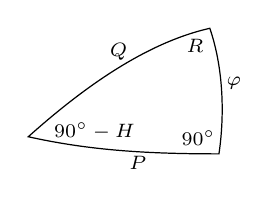
\begin{tikzpicture}[x=.145mm,y=-.145mm,line width=.44pt]
\draw (0,95) .. controls (47,53) and (102,13) .. (159,0)
  .. controls (171,35) and (172,76) .. (167,110)
  .. controls (104,110) and (54,107) .. (0,95) -- cycle;
\node[font=\scriptsize,inner sep=1pt] at (79,21) {\(Q\)};
\node[font=\scriptsize,inner sep=1pt] at (146,15) {\(R\)};
\node[font=\scriptsize,inner sep=1pt] at (180,48) {\(\varphi\)};
\node[font=\scriptsize,inner sep=1pt] at (58,90) {\(90^\circ-H\)};
\node[font=\scriptsize,inner sep=1pt] at (149,96) {\(90^\circ\)};
\node[font=\scriptsize,inner sep=1pt] at (96,118) {\(P\)};
\end{tikzpicture}\hfill\null\par
\ixeq{4)}{\operatorname{tang}P=\sin\varphi\operatorname{tang}R}
\ixeq{5)}{\operatorname{tang}Q=\frac{\operatorname{tang}\varphi}{\cos R}}
\ixeq{6)}{\operatorname{tang}H=\frac{\sin P}{\operatorname{tang}\varphi}.}
[Nun ist
\[
\begin{aligned}
\mathrm ds\,.\,\cos\zeta
&=\mathrm ds\,.\,\cos R\ixrad\frac{1-ee}{1-ee\cos H^2}
=\frac{a(1-ee)}{(1-ee\sin\varphi^2)^{\frac32}}\mathrm d\varphi\\
\mathrm ds\,.\,\sin\zeta
&=\mathrm ds\,.\,\sin R\ixrad\frac{1-ee\sin\varphi^2}{1-ee\cos H^2}
=\frac{a\cos\varphi}{(1-ee\sin\varphi^2)^{\frac12}}\mathrm d\lambda.
\end{aligned}
\]
\noindent Da aber
\[
\begin{aligned}
\cos R\,.\,\mathrm dQ&=\mathrm d\varphi\\
\sin R\,.\,\mathrm dQ&=\cos\varphi\,.\,\mathrm dP
\end{aligned}
\]
\noindent ist, so wird]
\[
\begin{aligned}
\frac{\mathrm ds}{a\,\mathrm dQ}
&=\frac{\surd(1-ee)\surd(1-ee\cos H^2)}
{(1-ee\sin\varphi^2)^{\frac32}}\\
\frac{\mathrm ds}{a\,\mathrm dQ}
&=\frac{\surd(1-ee\cos H^2)}{1-ee\sin\varphi^2}\frac{\mathrm d\lambda}{\mathrm dP},
\end{aligned}
\]
\noindent [also]
\par\smallskip
\noindent\textbf{IX.}\hfill 10\hspace{.12\textwidth}\par

% Printed 74; principal PDF 81; Google PDF 85.
\par\clearpage
\noindent\makebox[12mm][l]{\fontsize{13}{16}\selectfont 74}\makebox[\dimexpr\linewidth-24mm\relax][c]{\small\textbf{NACHLASS.}}\makebox[12mm][r]{}\par\medskip

\[
[\mathrm d\lambda=\ixrad\frac{1-ee}{1-ee\sin\varphi^2}\,.\,\mathrm dP
=\ixrad\frac{1-ee}{1-ee\sin\varphi^2}\,.\,\frac{\sin H}{\cos\varphi^2}\mathrm dQ
\]
\noindent oder wegen \(\sin\varphi=\cos H\sin Q\)]
\[
\mathrm ds=\frac{a\surd(1-ee)\surd(1-ee\cos H^2)}
{(1-ee\cos H^2\sin Q^2)^{\frac32}}\mathrm dQ
\]
\[
\left[\mathrm d\lambda=\frac{\surd(1-ee)\,.\,\sin H}
{(1-\cos H^2\sin Q^2)\surd(1-ee\cos H^2\sin Q^2)}\mathrm dQ\right].
\]

\bigskip
\begin{center}
[2.]\\[.5ex]
Kürzeste Linie auf dem Sphäroid.
\end{center}

\(\zeta\) Azimut, von Norden nach Osten gezählt.

Es sei
\[
\frac{\cos\varphi\sin\zeta}{\surd(1-ee\sin\varphi^2)}=\cos I,
\]
\noindent was konstant ist,
\[
\frac{\operatorname{tang}I}{\surd(1-ee)}=\operatorname{tang}i
\]
\noindent [\(i\) hat hier dieselbe Bedeutung wie vorher \(90^\circ-H\)]
\[
\frac{\operatorname{tang}\varphi}{\operatorname{tang}i}=\sin P,\qquad
\left[\frac{\sin\varphi}{\sin i}=\sin Q\right],
\]
\noindent so ist:
\[
\begin{aligned}
\cos P\sin I&=\cos\zeta\\
\cos P\sin i&=\cos R\\
\cos R&=\frac{\cos\zeta\surd(1-ee\sin i^2)}{\surd(1-ee)}\\
\sin R&=\frac{\sin\zeta\surd(1-ee\sin i^2)}{\surd(1-ee\sin\varphi^2)}\\
\operatorname{tang}R&=\frac{\operatorname{tang}\zeta\surd(1-ee)}{\surd(1-ee\sin\varphi^2)},
\end{aligned}
\]
\[
\begin{aligned}
\mathrm d\lambda&=\mathrm dP\ixrad\frac{1-ee}{1-ee\sin\varphi^2}\\
\mathrm ds&=a\,\mathrm dQ\frac{1-ee}{(1-ee\cos I^2)^{\frac12}(1-ee\sin\varphi^2)^{\frac32}}\\
&=a\,\mathrm dQ\frac{\surd(1-ee)\surd(1-ee\sin i^2)}
{(1-ee\sin\varphi^2)^{\frac32}}.
\end{aligned}
\]

% Printed 75; principal PDF 82; Google PDF 86.
\par\clearpage
\noindent\makebox[12mm][l]{}\makebox[\dimexpr\linewidth-24mm\relax][c]{\small\textbf{GEODÄTISCHE LINIE.}}\makebox[12mm][r]{\fontsize{13}{16}\selectfont 75}\par\medskip

\noindent [Da]
\[
\mathrm d\zeta=\mathrm ds\frac{\sin\zeta(1-ee\sin\varphi^2)^{\frac12}\operatorname{tang}\varphi}{a}
[=\mathrm d\lambda\,.\,\sin\varphi]
\]
\noindent [ist, so wird auch]
\[
\mathrm d\zeta=\mathrm dP\,.\,\sin\varphi\ixrad\frac{1-ee}{1-ee\sin\varphi^2}
\]
\noindent [oder wegen \(\mathrm dP\,.\,\sin\varphi=\mathrm dR\)]
\[
\mathrm d\zeta=\mathrm dR\ixrad\frac{1-ee}{1-ee\sin\varphi^2}.
\]
Man setze
\[
\ixrad\frac{1-ee\sin\varphi^2}{1-ee}=A
\]
\[
\frac{a\cos R}{\cos\zeta\surd(1-ee)}
=\frac a{\surd(1-ee)\surd(1-ee\cos I^2)}=\text{const.}=B,
\]
\noindent [so ist:]
\[
\begin{aligned}
\frac{\operatorname{tang}\zeta}{A}&=\operatorname{tang}R\\
\mathrm dQ&=\frac{A^3}{B}\mathrm ds\\
\mathrm d\lambda&=\frac{\mathrm dP}A\\
\mathrm d\zeta&=\frac{\mathrm dR}A.
\end{aligned}
\]

Zur indirekten Bestimmung von \(\varphi'-\varphi\), \(R'-R\) und \(\Delta P\) sind die folgenden
Formeln sehr bequem. Der Kürze halber wird
\[
\varphi^{*}=\tfrac12(\varphi+\varphi'),\qquad R^{*}=\tfrac12(R+R')
\]
\noindent geschrieben.

\noindent\hfill
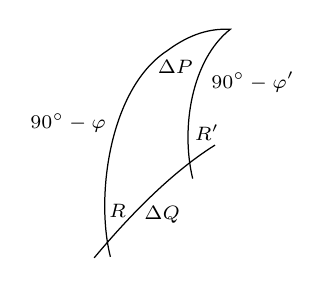
\begin{tikzpicture}[x=.129mm,y=-.129mm,line width=.45pt]
\draw (16,225) .. controls (1,166) and (15,59) .. (72,22)
  .. controls (95,5) and (115,0) .. (134,1)
  .. controls (96,31) and (85,98) .. (97,148);
\draw (0,226) .. controls (31,189) and (74,143) .. (119,115);
\node[font=\scriptsize,inner sep=1pt] at (80,38) {\(\Delta P\)};
\node[font=\scriptsize,inner sep=1pt,anchor=west] at (112,53) {\(90^\circ-\varphi'\)};
\node[font=\scriptsize,inner sep=1pt,anchor=east] at (15,93) {\(90^\circ-\varphi\)};
\node[font=\scriptsize,inner sep=1pt] at (111,103) {\(R'\)};
\node[font=\scriptsize,inner sep=1pt] at (23,180) {\(R\)};
\node[font=\scriptsize,inner sep=1pt] at (67,184) {\(\Delta Q\)};
\end{tikzpicture}\hfill\null\par
\[
\begin{aligned}
\varphi'-\varphi&=\alpha\,.\,\Delta Q\cos R^{*}\\
R'-R&=\beta\,.\,\Delta Q\sin R^{*}\operatorname{tang}\varphi^{*}\\
\Delta P&=\gamma\,.\,\frac{\Delta Q\sin R^{*}}{\cos\varphi^{*}}
\end{aligned}
\]
\noindent\hfill \(10^{*}\)\hspace{.12\textwidth}\par

% Printed 76; principal PDF 83; Google PDF 87.
\par\clearpage
\noindent\makebox[12mm][l]{\fontsize{13}{16}\selectfont 76}\makebox[\dimexpr\linewidth-24mm\relax][c]{\small\textbf{NACHLASS.}}\makebox[12mm][r]{}\par\medskip

\[
\begin{array}{@{}l@{\qquad}l@{}}
\begin{aligned}[t]
\log\alpha&=\frac{\mathrm{III}+2\mathrm{IV}}3\\[.4ex]
\log\beta&=\frac{\mathrm{III}+2\mathrm I}3\\[.4ex]
\log\gamma&=\frac{\mathrm{IV}-\mathrm I}3=\frac{\mathrm{III}-\mathrm{II}}3
\end{aligned}
&
\begin{array}[t]{@{}r@{\;}l@{}}
\mathrm{I}&=\log\sec\tfrac12\Delta Q\\
\mathrm{II}&=\log\sec\tfrac12(\varphi'-\varphi)\\
\mathrm{III}&=\log\sec\tfrac12(R'-R)\\
\mathrm{IV}&=\log\sec\tfrac12\Delta P\\
\multicolumn{2}{@{}l@{}}{\text{und zur Kontrolle: }\mathrm I+\mathrm{III}=\mathrm{II}+\mathrm{IV}.}
\end{array}
\end{array}
\]

\begin{center}Beispiel.\end{center}
[Gegeben sind \(\varphi\), \(\Delta s\) und \(\zeta\). Die Azimute sind in diesem Beispiel
von Süden nach Osten gezählt. Die Rechnung bezieht sich auf ein Ellipsoid, dessen
Abplattung \(\frac1{302{,}68}\) ist.]

\[
\begin{array}{@{}l@{\quad}r@{\;}l@{\quad}r@{\;}l@{\quad}r@{\;}l@{}}
\text{Kirchhesepe}&\varphi=&52^\circ\,37'\,32''{,}228&
\zeta=&284^\circ\,54'\,46''{,}185&R=&284^\circ\,55'\,48''{,}901\\
\text{Queckenberg}&\varphi'=&52\quad32\quad23{,}593&
\zeta'=&285\quad19\quad35{,}649&R'=&285\quad20\quad40{,}189\\
\cline{2-3}\cline{6-7}
&\varphi^*=&52\quad34\quad57{,}910&&&R^*=&285\qquad8\quad14{,}545
\end{array}
\]

{\small
\[
\renewcommand{\arraystretch}{1.16}
\begin{array}{@{}l@{\;}r@{\qquad}l@{\;}r@{\qquad}l@{\;}r@{}}
A\ \ldotp\,\ldotp\,\ldotp&0{,}000\,5306.81&
{[}\log a=&6{,}804\,5978&
\Delta Q\ \ldotp\,\ldotp\,\ldotp\,\ldotp&3{,}072\,5772\\
A'\ \ldotp\,\ldotp\,\ldotp&0{,}000\,5327.56&
\log\rho=&4{,}685\,5749]&
\cos R^*\ \ldotp\,\ldotp&9{,}416\,8638\\
\cline{6-6}
\operatorname{tang}\zeta\ \ldotp\,\ldotp&0{,}574\,5975_n&
\cos\zeta\ \ldotp\,\ldotp\,\ldotp&9{,}410\,5228&&2{,}489\,4410\\
1:A\ \ldotp\,\ldotp\,\ldotp&-5307&
\cos R\ \ldotp\,\ldotp\,\ldotp&9{,}411\,0183&
\alpha\ \ldotp\,\ldotp\,\ldotp\,\ldotp\,\ldotp\,\ldotp&+40\\
\cline{2-2}\cline{4-4}
\operatorname{tang}R\ \ldotp\,\ldotp&0{,}574\,0668_n&&-4955&
\multicolumn{2}{r}{-(\varphi'-\varphi)=308''{,}635}\\
\cline{5-6}\noalign{\vskip .45pt}\cline{5-6}
&&\dfrac{\surd(1-ee)}{a\rho}\ \ldotp\,\ldotp&8{,}508\,3901&
\Delta Q\ \ldotp\,\ldotp\,\ldotp\,\ldotp&3{,}072\,5772\\
\cline{4-4}
\mathrm I=&0{,}000\,0018&
1:B\ \ldotp\,\ldotp\,\ldotp\,\ldotp&8{,}507\,8946&
\sin R^*\ \ldotp\,\ldotp&9{,}984\,6634_n\\
\cline{6-6}
\mathrm{II}=&1&
{A^{*}}^3\ \ldotp\,\ldotp\,\ldotp\,\ldotp&+15952&&3{,}057\,2406_n\\
\cline{4-4}
\mathrm{III}=&29&&8{,}509\,4898&
\operatorname{tang}\varphi^*\ \ldotp\,\ldotp&0{,}116\,3188\\
\mathrm{IV}=&45&
\Delta s\ \ldotp\,\ldotp\,\ldotp\,\ldotp\,\ldotp&4{,}563\,0874&
\cos\varphi^*\ \ldotp\,\ldotp&9{,}783\,6284\\
\cline{4-4}\cline{6-6}
&&\Delta Q\ \ldotp\,\ldotp\,\ldotp\,\ldotp&3{,}072\,5772&&3{,}173\,5594_n\\
&&&&\beta\ \ldotp\,\ldotp\,\ldotp\,\ldotp\,\ldotp\,\ldotp&+22\\[1ex]
&&&&\multicolumn{2}{r}{R'-R=1491''{,}288}\\
\cline{5-6}\noalign{\vskip .45pt}\cline{5-6}
&&R'-R\ \ldotp\,\ldotp&3{,}173\,5616&&3{,}273\,6122\\
&&\Delta P\ \ldotp\,\ldotp\,\ldotp\,\ldotp&3{,}273\,6131&
\gamma\ \ldotp\,\ldotp\,\ldotp\,\ldotp\,\ldotp\,\ldotp&+9\\
&&1:A^*\ \ldotp\,\ldotp\,\ldotp&-5317&
\multicolumn{2}{r}{\Delta P=1877''{,}643}\\
\cline{4-4}\cline{5-6}\noalign{\vskip .45pt}\cline{5-6}
&&\multicolumn{2}{r}{\zeta'-\zeta=1489''{,}464}&&\\
\cline{3-4}\noalign{\vskip .45pt}\cline{3-4}
&&\lambda=&1875''{,}346&&\\
&&=&31'\,15''{,}346&&\\
\cline{3-4}\noalign{\vskip .45pt}\cline{3-4}
\end{array}
\]
\par
}

% Printed 77; principal PDF 84; Google PDF 88.
\par\clearpage
\noindent\makebox[12mm][l]{}\makebox[\dimexpr\linewidth-24mm\relax][c]{\small\textbf{GEODÄTISCHE LINIE.}}\makebox[12mm][r]{\fontsize{13}{16}\selectfont 77}\par\medskip

Alle diese Vorschriften lassen sich durch viel einfachere ersetzen,
wenn man die wahren Azimute beibehält und veränderte Polhöhen \(\psi\) einführt,
sodass \(\operatorname{tang}\psi=\surd(1-ee)\,.\,\operatorname{tang}\varphi\) gilt.

\begin{center}
Hilfstafel für \(\mathrm C\,.\log\surd(1-ee\sin\varphi^2)\);
\(\mathrm C\,.\log\surd(1-ee)=14372.073\)\\
{[in Einheiten der 7. Dezimalstelle].}
\end{center}

\noindent\hfill
{\small\setlength{\tabcolsep}{4.5pt}\renewcommand{\arraystretch}{1.12}%
\begin{tabular}{@{}rr|r||rr|r||rr|r||rr|r@{}}
\hline
\(48^\circ\)&\(0'\)&7925.420&\(50^\circ\)&\(0'\)&8422.342&\(52^\circ\)&\(0'\)&8913.294&\(54^\circ\)&\(0'\)&9395.884\\
&4&42.053&&4&&&4&29.528&&4&\\
&8&58.683&&8&55.284&&8&45.753&&8&9427.701\\
&12&75.309&&12&71.745&&12&61.969&&12&\\
&16&7991.932&&16&8488.200&&16&78.175&&16&59.469\\
\hline
&20&8008.550&&20&8504.648&&20&8994.371&&20&\\
&24&25.163&&24&21.088&&24&9010.558&&24&9491.188\\
&28&41.772&&28&37.521&&28&26.735&&28&\\
&32&58.376&&32&53.947&&32&42.902&&32&9522.856\\
&36&74.976&&36&70.366&&36&59.059&&36&\\
\hline
&40&8091.571&&40&8586.777&&40&75.205&&40&54.474\\
&44&8108.162&&44&8603.180&&44&9091.341&&44&\\
&48&24.748&&48&19.576&&48&9107.467&&48&9586.042\\
&52&41.329&&52&35.964&&52&23.583&&52&9601.806\\
&56&57.904&&56&52.344&&56&39.688&&56&17.557\\
\hline
49&0&74.475&51&0&68.716&53&0&55.783&55&0&33.296\\
&4&8191.040&&4&8685.080&&4&71.868&&4&49.022\\
&8&8207.599&&8&8701.436&&8&9187.941&&8&64.734\\
&12&24.154&&12&17.784&&12&9204.004&&12&80.433\\
&16&40.703&&16&34.124&&16&20.056&&16&9696.119\\
\hline
&20&57.246&&20&50.455&&20&36.097&&20&9711.791\\
&24&73.783&&24&66.778&&24&52.127&&24&27.450\\
&28&8290.315&&28&83.092&&28&68.146&&28&9743.095\\
&32&8306.840&&32&8799.398&&32&9284.154&&&\\
&36&23.360&&36&8815.695&&36&9300.150&&&\\
\hline
&40&39.876&&40&31.984&&40&16.135&&&\\
&44&56.385&&44&48.264&&44&32.108&&&\\
&48&&&48&64.535&&48&&&&\\
&52&8389.374&&52&80.797&&52&64.019&&&\\
&56&&&56&8897.050&&56&&&&\\
\hline
50&0&8422.342&52&0&8913.294&54&0&9395.884&&&
\end{tabular}}\hfill\null\par

\begin{center}
[Dieser Tafel liegt die Abplattung \(\frac1{302{,}68}\) zugrunde.]
\end{center}

% Printed 78; principal PDF 85; Google PDF 89.
\par\clearpage
\noindent\makebox[12mm][l]{\fontsize{13}{16}\selectfont 78}\makebox[\dimexpr\linewidth-24mm\relax][c]{\small\textbf{NACHLASS.}}\makebox[12mm][r]{}\par\medskip

\begin{center}
[3.]\\[.5ex]
Geodätische Linie.
\end{center}
\begin{quote}
\noindent \(\varphi\) \ixpoints{4} Breite\\
{[}\(\psi\) \ixpoints{4} reduzierte Breite]\\
\(\lambda\) \ixpoints{4} Länge\\
\(\left.
\begin{array}{@{}l@{}}
\zeta\ \text{\ixpoints{4} [von Süden nach Osten gezähltes] Azimut}\\
s\ \text{\ixpoints{4} Länge}
\end{array}
\right\}\ \text{[der geodätischen Linie]}\)\\
{[}\(a\) \ixpoints{4} große Halbachse\\
\(e\) \ixpoints{4} Exzentrizität].
\end{quote}
\[
\begin{aligned}
\surd(1-ee)\,.\,\operatorname{tang}\varphi&=\operatorname{tang}\psi\\
\frac{\cos\varphi}{\surd(1-ee\sin\varphi^2)}&=\cos\psi\\
\sin\varphi\ixrad\frac{1-ee}{1-ee\sin\varphi^2}&=\sin\psi\\
(1-ee\sin\varphi^2)(1-ee\cos\psi^2)&=1-ee\\
\frac{\mathrm d\varphi}{\sin\varphi\cos\varphi}
&=\frac{\mathrm d\psi}{\sin\psi\cos\psi}\\
\frac{\surd(1-ee)}{1-ee\sin\varphi^2}\mathrm d\varphi&=\mathrm d\psi.
\end{aligned}
\]
\noindent [Es ist]
\[
\begin{aligned}
\frac{\cos\varphi\sin\zeta}{\surd(1-ee\sin\varphi^2)}&=\cos I=\text{const.}\\
\mathrm d\lambda
\left[=\mathrm ds\,.\,\sin\zeta\frac{\surd(1-ee\sin\varphi^2)}{a\cos\varphi}\right]
&=\frac{\mathrm ds\,.\,\sin\zeta}{a\cos\psi}\\
-\mathrm d\varphi
&=\mathrm ds\,.\,\cos\zeta\frac{(1-ee\sin\varphi^2)^{\frac32}}{a(1-ee)}\\
-\mathrm d\psi&=\frac{\mathrm ds\,.\,\cos\zeta}{a\surd(1-ee\cos\psi^2)}.
\end{aligned}
\]
Es sei
\[
\mathrm d\sigma=\frac{\mathrm ds}{a\surd(1-ee\cos\psi^2)},\qquad
\mathrm dl=\frac{\mathrm d\lambda}{\surd(1-ee\cos\psi^2)},
\]
\noindent so wird
\[
\mathrm dl=\frac{\mathrm d\sigma\,.\,\sin\zeta}{\cos\psi},\qquad
-\mathrm d\psi=\mathrm d\sigma\,.\,\cos\zeta.
\]
\noindent [Da]
\ixeq{1)}{\cos\psi\sin\zeta=\cos I,}
\noindent [so ist]
\par

% Printed 79; principal PDF 86; Google PDF 90.
\par\clearpage
\noindent\makebox[12mm][l]{}\makebox[\dimexpr\linewidth-24mm\relax][c]{\small\textbf{GEODÄTISCHE LINIE.}}\makebox[12mm][r]{\fontsize{13}{16}\selectfont 79}\par\medskip

\[
\begin{aligned}
\mathrm d\sigma
&=-\frac{\mathrm d\psi\,.\,\cos\psi}{\surd(\cos\psi^2-\cos I^2)}
=-\frac{\mathrm d\sin\psi}{\surd(\sin I^2-\sin\psi^2)}\\
\sigma&=\operatorname{arc\,cos}\frac{\sin\psi}{\sin I}+\text{const.}
\end{aligned}
\]
\noindent Setzt man die Konstante \(=0\), so erhält man
\ixeq{2)}{\sin\psi=\cos\sigma\sin I}
\noindent [und daher]
\ixeq{3)}{\operatorname{cotang}I=\operatorname{tang}\zeta\sin\sigma.}
\noindent [Weiter ist]
\[
\begin{aligned}
\mathrm dl&=-\frac{\mathrm d\psi}{\cos\psi}\operatorname{tang}\zeta
=-\frac{\mathrm d\psi\,.\,\cos I}{\cos\psi\surd(\cos\psi^2-\cos I^2)}\\
&=-\frac{\operatorname{cotang}I\,.\,\mathrm d\operatorname{tang}\psi}
{\surd(1-\operatorname{cotang}I^2\operatorname{tang}\psi^2)}.\\
l&=\operatorname{arc\,cos}(\operatorname{cotang}I\operatorname{tang}\psi)+\text{const.}
\end{aligned}
\]
\noindent Setzt man also die Konstante \(=0\), so erhält man
\ixeq{4)}{\operatorname{tang}\psi=\operatorname{tang}I\cos l,}
\noindent [folglich]
\ixeq{5)}{\sin\sigma=\sin l\cos\psi}
\ixeq{6)}{\operatorname{tang}l=\frac{\operatorname{tang}\sigma}{\cos I}.}
\noindent [Mithin wird]
\ixeq{7)}{\mathrm dl=\frac{\cos I}{\cos\psi^2}\mathrm d\sigma
=\frac{\cos l^2}{\cos\sigma^2\cos I}\mathrm d\sigma.}

\noindent Das Integral \(\int\mathrm ds\) erhält man leicht aus 2 und das Integral \(\int\mathrm d\lambda\)
aus 2 und 7, nämlich
\[
\begin{gathered}
{[}\mathrm d\lambda=(1-ee\cos\psi^2)^{\frac12}\mathrm dl
=(1-\tfrac12 ee\cos\psi^2-\tfrac18e^4\cos\psi^4-\ldots)\mathrm dl]\\
\mathrm d\lambda=\mathrm dl-\tfrac12ee\cos I\,.\,\mathrm d\sigma
\{1+\tfrac14 ee(1-\cos\sigma^2\sin I^2)+\text{etc.}\}\\
\left[\frac{\mathrm ds}a=\mathrm d\sigma-\tfrac12ee(1-\cos\sigma^2\sin I^2)\mathrm d\sigma
\{1+\tfrac14 ee(1-\cos\sigma^2\sin I^2)+\text{etc.}\}\right].
\end{gathered}
\]

% Printed 80; principal PDF 87; Google PDF 91.
\par\clearpage
\noindent\makebox[12mm][l]{\fontsize{13}{16}\selectfont 80}\makebox[\dimexpr\linewidth-24mm\relax][c]{\small\textbf{NACHLASS.}}\makebox[12mm][r]{}\par\medskip

\bigskip
\begin{center}
[Geodätische Übertragung von Breite, Länge und Azimut.]\\[.8ex]
{[4.]}
\end{center}
[Es bezeichne \(\rho\) die Länge des Bogens von einer Sekunde in Einheiten des
Radius, \(M\) den Modul des gewählten Logarithmensystems, ferner \(a\) die
große Halbachse der Meridianellipse des Rotationsellipsoids und \(e\) deren
Exzentrizität. Weiter sei
\[
\begin{alignedat}{2}
\tfrac1{12}M\rho\rho&=\mu &\qquad \frac{\mu}{1-ee}&=E\\
\frac1{a\rho(1-ee)}&=A &\qquad \frac{M}{12aa(1-ee)}&=F\\
\frac1{a\rho}&=B &\qquad \frac{Mee}{12aa(1-ee)}&=G\\
\frac{\mu}{2(1-ee)}&=C &\qquad \tfrac32 ee\mu&=H\\
\frac{\mu(1-ee)}2&=D &\qquad \tfrac52 ee\mu&=I]
\end{alignedat}
\]
\[
\begin{aligned}
\frac1{1-ee\sin\varphi^2}&=QQ\\
\frac A{Q^3}&=A'\\
\frac BQ&=B'\\[.5ex]
C(1-3ee+2ee\sin\varphi^2)&=C'\\
DQ^4(1-8ee\sin\varphi^2)&=D'\\[.5ex]
\frac E{QQ}&=E'\\
\frac F{QQ}&=F'\\
\frac{G\sin\varphi^2}{QQ}&=G'\\[.5ex]
HQ^4(1-(2-4ee)\sin\varphi^2-3ee\sin\varphi^4)&=H'\\
IQ^4\left(1+\frac{2-12ee}{5}\sin\varphi^2+ee\sin\varphi^4\right)&=I'.
\end{aligned}
\]
\noindent [Sind \(\Delta\varphi\), \(\Delta\zeta\), \(\Delta\lambda\) die Breiten-, Azimut- und Längendifferenzen
des Anfangs- und Endpunkts der geodätischen Linie \(s\) sowie \(\varphi\) und \(\zeta\)
die arithmetischen Mittel der Breiten und Azimute an beiden Punkten, so gilt:]
\par

% Printed 81; principal PDF 88; Google PDF 92.
\par\clearpage
\noindent\makebox[12mm][l]{}\makebox[\dimexpr\linewidth-24mm\relax][c]{\small\textbf{GEODÄTISCHE LINIE.}}\makebox[12mm][r]{\fontsize{13}{16}\selectfont 81}\par\medskip

\[
\begin{alignedat}{2}
\Delta\varphi&=A'\,.\,s\cos\zeta
&\,.\,\text{Zahl}\log&(E'\Delta\lambda^2+C'\Delta\zeta^2-H'\Delta\varphi^2)\\
\Delta\zeta&=B'\,.\,s\sin\zeta\operatorname{tang}\varphi
&\,.\,\text{Zahl}\log&(F'ss+C'\Delta\zeta^2+I'\Delta\varphi^2)\\
\Delta\lambda&=B'\,.\,s\frac{\sin\zeta}{\cos\varphi}
&\,.\,\text{Zahl}\log&(G'ss+C'\Delta\zeta^2-D'\Delta\varphi^2).
\end{alignedat}
\]
\noindent [Die Koeffizienten \(A'\), \(B'\), \(C'\), \(D'\) usw. haben als Argument \(\varphi\).]

\begin{center}
[Beispiel.]\\[.5ex]
{[Übertragung der geografischen Koordinaten von Göttingen, Sternwarte, 1,
zum Hauptdreieckspunkt Hohehagen, 3. Die Azimute sind hier
von Süden nach Westen gezählt. Die Länge ist nach Westen positiv.]}
\end{center}
\[
\begin{array}{@{}r@{\;}l@{\qquad}r@{\;}l@{}}
51^\circ\,31'\,48''{,}1782&=\varphi_1&64^\circ\phantom{0}\,1'\,17''{,}5880&=\zeta_1\\
51\quad28\quad31{,}3844&=\varphi_3&243\quad52\quad52{,}6744&=\zeta_3\\
\hline
51\quad30\qquad9{,}7813&=\varphi&63\quad57\qquad5{,}1312&=\zeta\\
-3\quad16{,}7938&=\Delta\varphi&-8\quad24{,}9136&=\Delta\zeta
\end{array}
\]

{\small
\[
\renewcommand{\arraystretch}{1.1}
\begin{array}{@{}l@{\;}r@{\qquad}l@{\;}r@{\qquad}r@{}}
s\ \ixmathdots{5}&4{,}141\,3507&&&\\
A'\ \ixmathdots{5}&8{,}510\,0643&&&\\
B'\ \ixmathdots{5}&8{,}508\,9486&&&\\
\cline{2-2}
A's\ \ixmathdots{4}&2{,}651\,4150&B's\ \ixmathdots{5}&2{,}650\,2993&\\
\cos\zeta\ \ixmathdots{3}&9{,}642\,5960&\sin\zeta\ \ixmathdots{4}&9{,}953\,4804&\\
\cline{2-2}\cline{4-4}
&2{,}294\,0110&&2{,}603\,7797&\\
&+5&\operatorname{tang}\varphi\ \ixmathdots{3}&0{,}099\,4371&\\
\multicolumn{2}{r}{-\Delta\varphi=196''{,}7938}&
\cos\varphi\ \ixmathdots{4}&9{,}794\,1237&\\
\cline{1-2}\cline{4-4}\noalign{\vskip .45pt}\cline{1-2}
&&&2{,}703\,2168&2{,}809\,6560\\
&&&+3&+1\\
&&\multicolumn{2}{r}{-\Delta\zeta=504''{,}9136}&
\Delta\lambda=645''{,}1431\\
\cline{3-4}\cline{5-5}\noalign{\vskip .45pt}\cline{3-4}\cline{5-5}
\end{array}
\]
\[
\begin{array}{@{}l@{\quad}l@{\quad}l@{\quad}l@{}}
ss\ \ixmathdots{4}\ 8{,}28270&
\Delta\varphi^2\ \ixmathdots{3}\ 4{,}58802&
\Delta\zeta^2\ \ixmathdots{3}\ 5{,}40643&
\Delta\lambda^2\ \ixmathdots{3}\ 5{,}61931\\
\hline
F'\ \ixmathdots{4}\ 1{,}95052&
-D'\ \ixmathdots{3}\ 4{,}61510_n&
C'\ \ixmathdots{4}\ 4{,}62648&
E'\ \ixmathdots{4}\ 4{,}93087\\
G'\ \ixmathdots{4}\ 9{,}55683&
\phantom{-}I'\ \ixmathdots{3}\ 3{,}24304&&\\
&-H'\ \ixmathdots{3}\ 2{,}26361&&
\end{array}
\]
\[
\begin{alignedat}{3}
-H'\Delta\varphi^2&=0.000
&\qquad F'ss&=1.711
&\qquad G'ss&=\phantom{-}0.007\\
C'\Delta\zeta^2&=1.079
&\qquad I'\Delta\varphi^2&=0.007
&\qquad -D'\Delta\varphi^2&=-0.160\\
E'\Delta\lambda^2&=3.550
&\qquad C'\Delta\zeta^2&=1.079
&\qquad C'\Delta\zeta^2&=\phantom{-}1.079
\end{alignedat}
\]
\par
}
\noindent\textbf{IX.}\hfill 11\hspace{.12\textwidth}\par
\par
\endgroup
